\chapter{Конструкторская часть}

В данном разделе будут представлены схемы алгоритмов поиска редакционного расстояния, среди которых матричная реализация алгоритма вычисления расстояния Левенштейна и три реализации алгоритма вычисления расстояния Дамерау~--~Левенштейна: матричная, рекурсивная и рекурсивная с кэшированием.

\section{Разработка матричной реализации алгоритма нахождения расстояния Левенштейна}
На рисунках \ref{img:lev01}~--~\ref{img:lev02} представлена схема матричного алгоритма нахождения расстояния Левенштейна.

\begin{figure}[h!]
\centering
    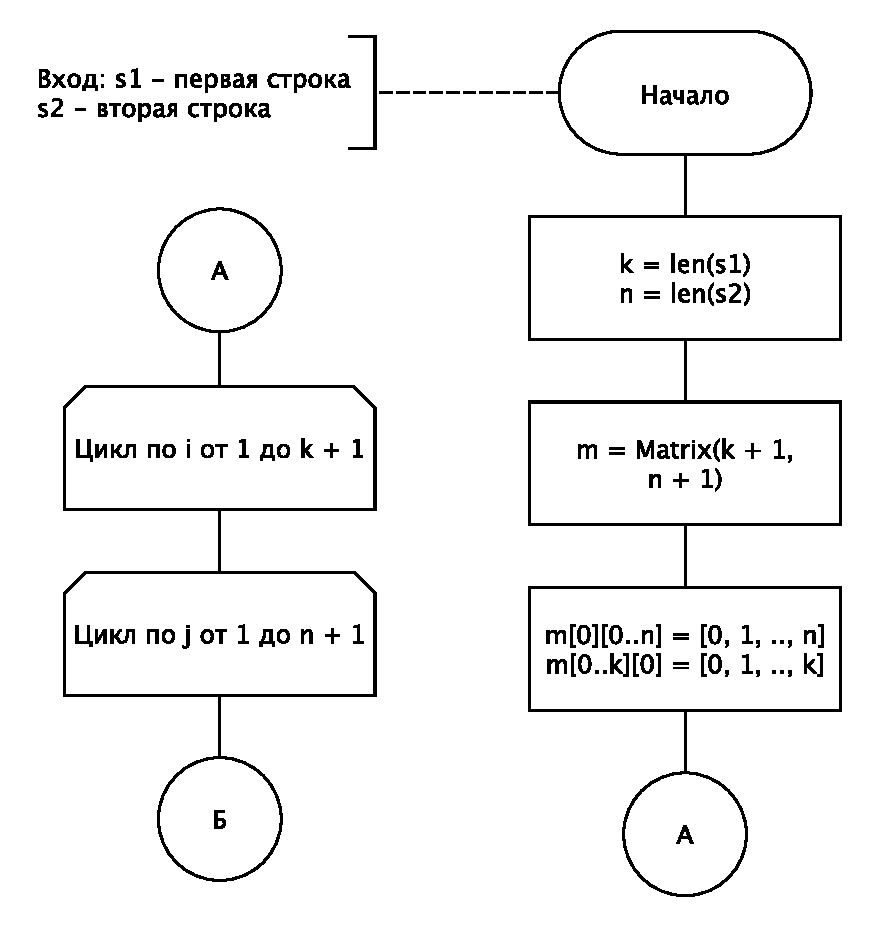
\includegraphics[width=0.55\linewidth]{levenshtein01.pdf}
    \caption{Схема матричной реализации алгоритма нахождения расстояния Левенштейна}
    \label{img:lev01}	
\end{figure}

\newpage

\begin{figure}[h!]
    \centering
    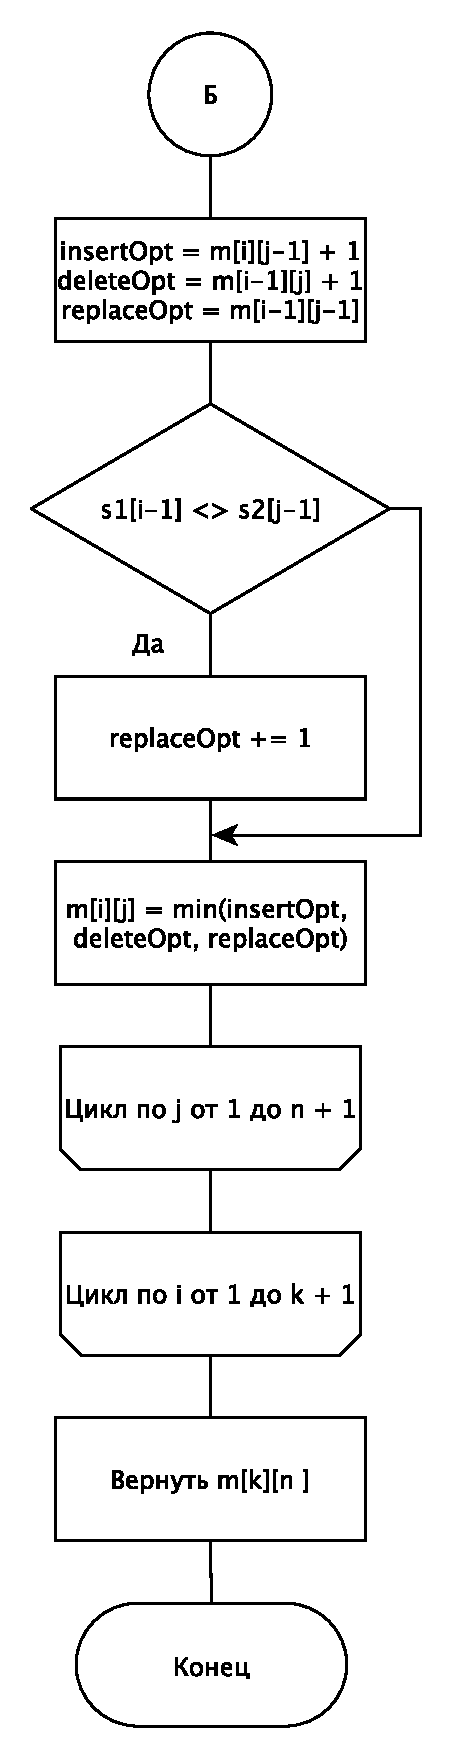
\includegraphics[width=0.3\linewidth]{levenshtein02.pdf}
    \caption{Схема матричной реализации нахождения расстояния Левенштейна (продолжение рис.~\ref{img:lev01})}
    \label{img:lev02}
\end{figure}

\newpage

\section{Разработка матричной реализации алгоритма нахождения расстояния Дамерау~--~Левенштейна}
На рисунке \ref{img:dam_lev} представлена схема матричной реализации алгоритма нахождения расстояния Дамерау~--~Левенштейна. 

\begin{figure}[h!]
    \centering
    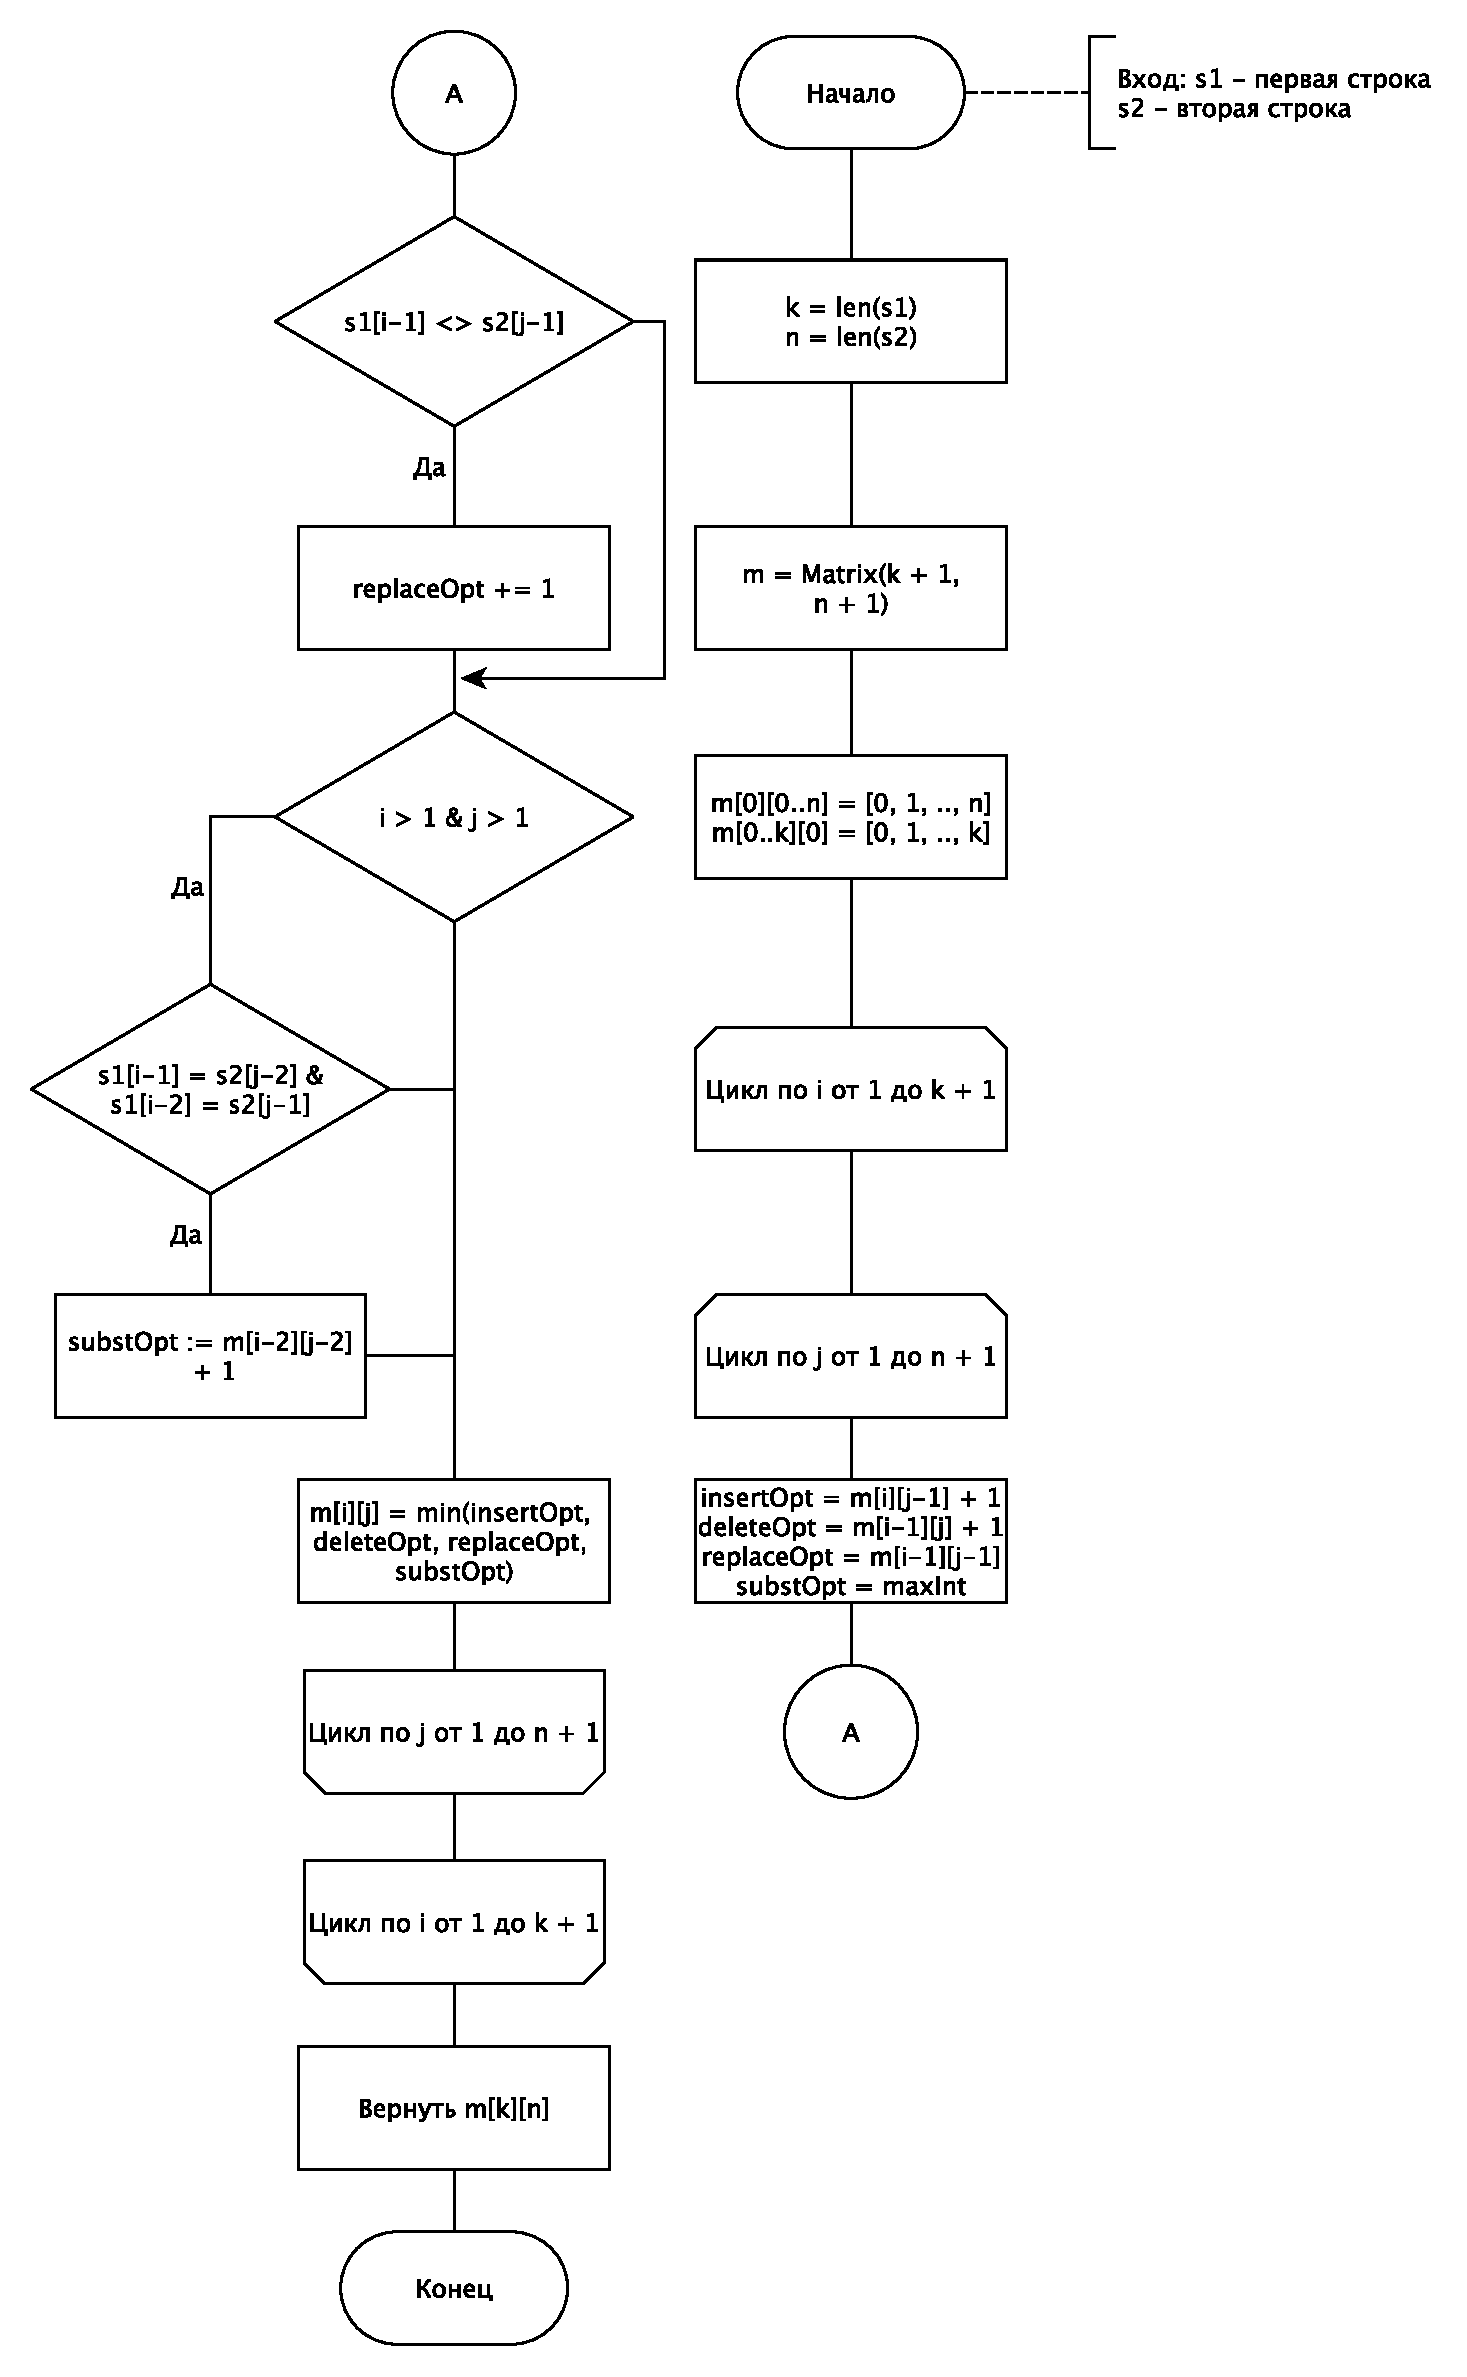
\includegraphics[width=0.6\linewidth]{dam_lev.pdf}
    \caption{Схема матричной реализации алгоритма нахождения расстояния Дамерау~--~Левенштейна}
    \label{img:dam_lev}
\end{figure}

\section{Разработка рекурсивной реализации алгоритма нахождения расстояния Дамерау~--~Левенштейна}
На рисунке \ref{img:rec_dam_lev} представлена схема рекурсивной реализации алгоритма нахождения расстояния Дамерау~--~Левенштейна.

\begin{figure}[h!]
    \centering
    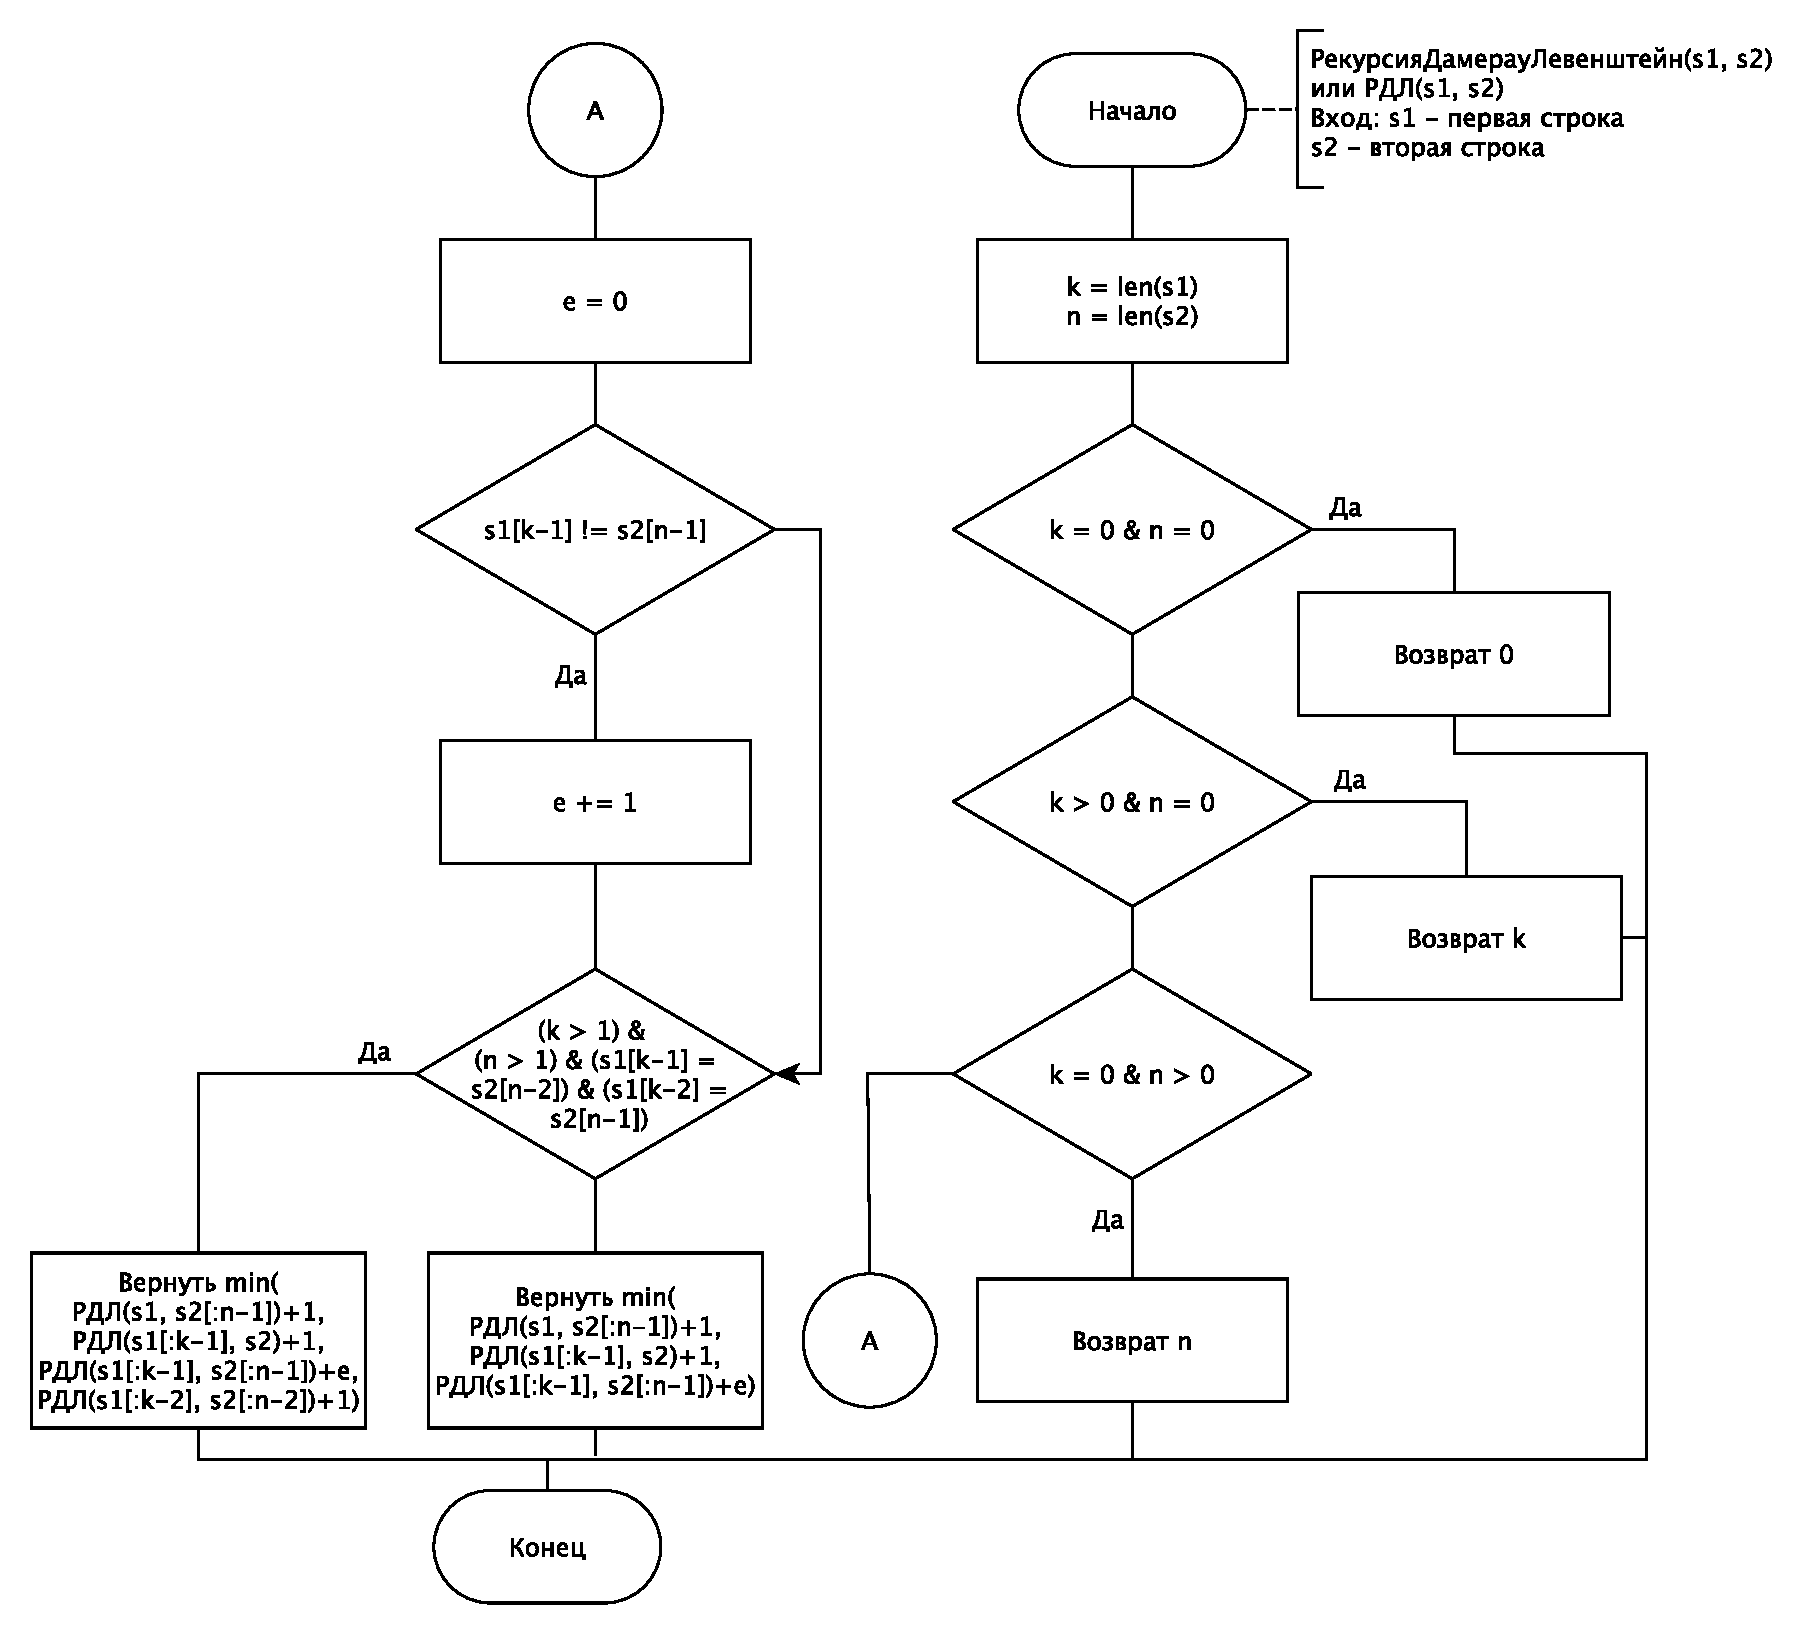
\includegraphics[width=1\linewidth]{rec_dam_lev.pdf}
    \caption{Схема рекурсивной реализации алгоритма нахождения расстояния Дамерау~--~Левенштейна}
    \label{img:rec_dam_lev}
\end{figure}

\section{Разработка рекурсивной реализации алгоритма нахождения расстояния Дамерау~--~Левенштейна с кэшем}
На рисунке \ref{img:rec_dam_lev_cache} представлена схема рекурсивной реализации алгоритма нахождения расстояния Дамерау~--~Левенштейна с кэшем.

\begin{figure}[h!]
    \centering
    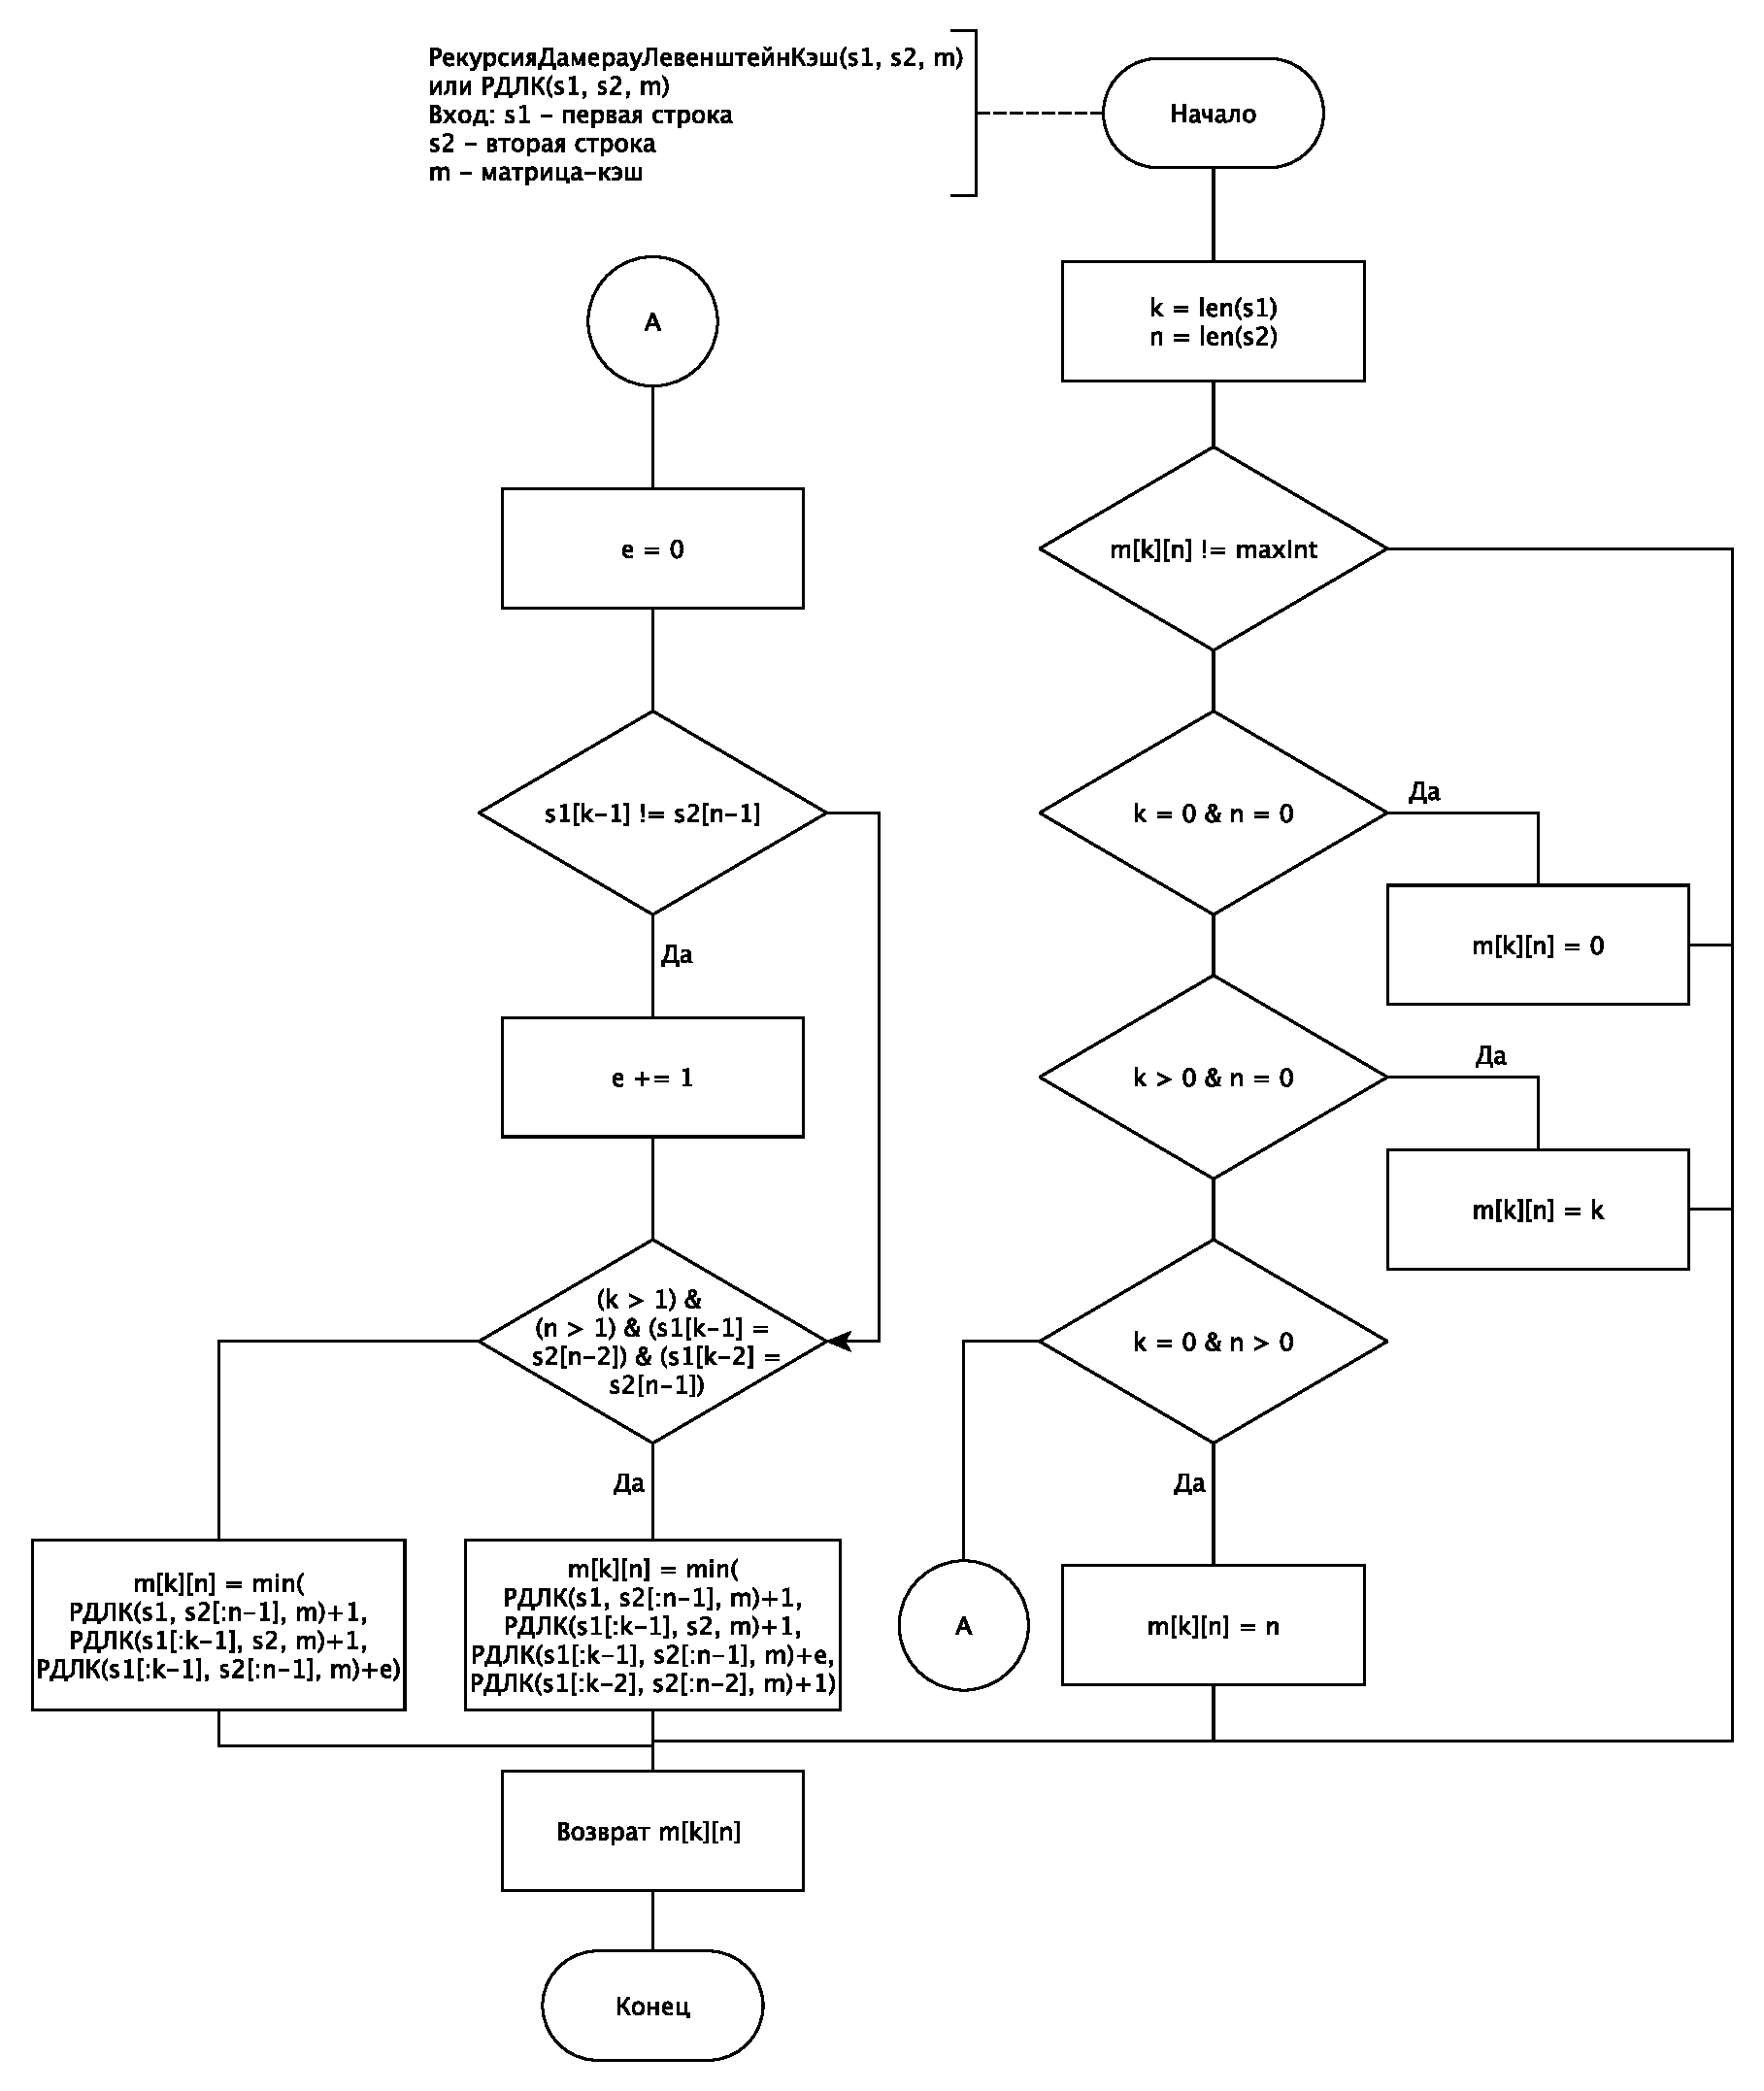
\includegraphics[width=0.85\linewidth]{rec_dam_lev_cache.pdf}
    \caption{Схема рекурсивной реализации алгоритма нахождения расстояния Дамерау~--~Левенштейна с кэшем}
    \label{img:rec_dam_lev_cache}
\end{figure}

\newpage